

%--------------------------------

\newpage


\section{Gamed-based tools as media to transmit freshwater ecology concepts}{Communication scientifique par la gamification}

\label{app:sec:mediationecotox}


% illustration of sci communication


\bpar{
The issue of scientific communication, in particular between agents producing knowledge, has been a recurrent theme in our work. It also plays a role in the interface with the public for scientific mediation, and the development of a mediation can in return inform interdisciplinary enterprises. We develop here two models as games, with a similar objective to transmit freshwater ecology concepts. This reinforces the idea of the model as a crucial instrument of scientific mediation.
}{
La question de la communication scientifique, notamment entre les agents producteurs de connaissance, a été un thème récurrent de notre travail. Celle-ci intervient également dans le contact avec le public comme médiation scientifique, et le développement d'une médiation peut en retour informer les entreprises d'interdisciplinarité. Nous développons ici deux modèles sous forme de jeux, ayant un objectif similaire de transmettre des concepts d'écologie aquatique. Cela renforce l'idée du modèle comme instrument crucial de la médiation scientifique.
}


\stars


\bpar{
\textit{This section is the output of an interdisciplinary collaboration with the ecotoxicologist \noun{Dr. Hélène Serra} (Université de Bordeaux and Ineris) and was presented at the SETAC 2016 conference as~\cite{serra:halshs-01322860}.}
}{
\textit{Cette section est le fruit d'une collaboration interdisciplinaire avec l'écotoxicologue \noun{Dr. Hélène Serra} (Université de Bordeaux et Ineris) et a été présentée à la conférence SETAC 2016 comme~\cite{serra:halshs-01322860}.}
}

\stars

%--------------------------------


\subsection{Introduction}{Introduction}

\bpar{
There is an increasing expectation on people to be aware and to get involved in the environmental issues that our world is facing. However, expert knowledge is often required to understand most of these issues. One of the challenges in science today lies in explaining complex issues in a simple and understandable way to an unspecialized audience. Games can turn out to be a good medium for scientific vulgarization. Indeed, the first form of learning we all experienced was by playing. Games are very popular, and from an educational point of view, they present many advantages. They are dynamic and interactive. Therefore, the player engagement increases, as well as its knowledge retention. In addition, the player is immerged into a new world and discovers a virtual environment where he needs to develop strategies and to identify crucial processes. Those characteristics can be wisely used to spread scientific topics, and gamification has already been proposed as a tool for an easier propagation of scientific thinking~\cite{morris2013gaming} such as in pharmacology~\cite{cain2015serious} or geosciences~\cite{reynard2015application}. In this context, our project aims at developing game-based tools to transmit the basic concepts of freshwater ecology. We choose to focus on a classical board game and on a computer based game because they are complementary in the targeted audience (groups versus online gamers) and the possibilities offered, in particular regarding the interactions between players and the system dynamics. 
}{
L'attente de prise de conscience et d'implication du public concernant les questions environnementales est croissante. Toutefois, une connaissance experte est souvent nécessaire pour comprendre le enjeux sous-jacents à la plupart de ces problèmes. L'un des défis de la science aujourd'hui réside dans le fait d'expliquer des questions complexes de façon simple et compréhensible à une audience non-spécialisée. Les jeux apparaissent comme un moyen pertinent pour la vulgarisation scientifique. En effet, la première forme d'apprentissage est en général par le jeu. Les jeux sont très populaires et présentent divers avantages d'un point de vue éducatif. Ceux-ci sont dynamiques et interactifs. Ainsi, l'engagement du joueur est augmenté, ainsi que sa rétention de connaissances. De plus, le joueur est immergé dans un monde nouveau et découvre un environnement virtuel où il doit développer des stratégies et identifier les processus fondamentaux. Ces caractéristiques peuvent être aisément utilisées pour transmettre des concepts scientifiques, et la gamification a déjà été proposée comme un outil pour une meilleure propagation de la pensée scientifique~\cite{morris2013gaming} comme en pharmacologie~\cite{cain2015serious} ou les géosciences~\cite{reynard2015application}. Dans ce contexte, ce projet vise à développer des outils basés sur les jeux pour transmettre des concepts basiques en écologie aquatique. Nous nous intéressons à un jeu de plateau classique et à un jeu informatique car ceux-ci sont complémentaires dans l'audience visée (joueurs en groupe et joueurs en ligne) et dans les possibilités offertes, en particulier concernant les interactions entre joueurs et les dynamiques du système. 
}

% There is an increasing awarness of the public on environmental issues
% Expert knowledge is often required to understand them
% A need for simple and understandable tools to explain environmental issues
% Games provide a virtual world with given boundaries (rules) that the player needs to understand and to follow to win
% Furthermore, games are dynamic and interactive: the player engagementanditsknowledgeretentionincrease
% Games display interesting features to spread scientific thinking1

%Objective : TO DEVELOP A BOARD GAME AND A COMPUTER-BASED GAME TO EXPLAIN THE BASIC CONCEPTS OF AQUATIC ECOLOGY
% The games aim to be complementary:
% - in term of player interactions and system dynamics
% - inthetargetedplayers(groupsvsisolated gamers) 


\subsection{Material and Methods}{Méthodologie}

\bpar{
The general methodology is divided in five steps: (1) selection of species; (2) definition of the instructions (object, game board, rules); (3) incorporation of environmental stressors (biotic and abiotic), (4) design and construction of interfaces (board and computer model); (5) test with players. All steps are necessarily interdependent and are tackled in parallel during the development of the games.
}{
La méthodologie pour la conception des deux types de jeux est divisée de manière similaire en 5 étapes : (1) sélection des espèces ; (2) définition des instructions (objets, environnement du jeu, règles) ; (3) inclusion des stress environnementaux (biotiques et abiotiques) ; (4) conception et construction des interfaces (plateau et implémentation informatique) ; (5) test avec des joueurs. L'ensemble des étapes sont interdépendantes et sont menées en parallèle pendant le développement des jeux.
}

% methodo poster
% 1) Context : Aim of the games ; Aquatic species and ecological concepts ; Inclusion of time and chance
% 2) Prototypes : Design of the games (players , token, board) ; Size and layout of the board ; Coding and calibration of the model
% 3) Test and evaluation : Gather player feedbacks, Refining and adapting the games
% 4) Diffusion : Identification of funding opportunities ; Construction of a diffusion network


\bpar{
While the board game is inspired by past experiences of player, the computer game is based on a model of simulation of the ecosystem. In order to introduce notions of equilibrium and its perturbations that occur at a larger time scale than on the board game, we propose to implement an agent-based model (ABM) and to couple its dynamics with gaming actions. ABM have already been widely used in ecology~\cite{grimm2005pattern}. Therefore, we selected a trophic chain dynamic model (extended prey-predator model) that can capture fish behavioral rules and spatially heterogeneous environment. It is particularly suitable for the game implementation: fish behaviors are influenced by players whereas the ecosystem is disturbed by external events. 
}{
Tandis que le jeu de plateau est inspiré d'experiences de joueurs, le jeu informatique se base sur un modèle de simulation de l'écosystème. De manière à introduire les notions d'équilibre et ses perturbations qui surviennent à une échelle de temps plus longue que celle du jeu de plateau, nous proposons d'implémenter un modèle basé-agent (ABM) et de coupler sa dynamique avec des actions de jeu. Les ABM sont déjà largement utilisés en écologie~\cite{grimm2005pattern}. Ainsi, nous choisissons un modèle dynamique de chaine trophique (modèle proie-prédateur étendu) qui est capable d'inclure des règles comportementales pour les poissons et un environnement spatial hétérogène. Un tel modèle est particulièrement adapté pour l'implémentation du jeu : les comportements des poissons sont influencés par les joueurs tandis que l'écosystème est perturbé par des évènements extérieurs.
}


\subsection{Results}{Résultats}

% Table 1 gives an overview on how the game can be introduced to a specific audience:
% ``You, little fish, just reached a new lake after an extremely intense rain event. This new area is to be conquered. But you are not the only one: three other fish species just arrived. Which player will find its territory first? Which of you will reproduce fast enough to reach a stable population and therefore remain forever and ever in the lake? Be careful! Nature is often hostile and might stay in your way. You will need to use strategy to avoid enemies; to compete for resources, to grow up and eventually you will reproduce \ldots and become the next master of water!''

\bpar{
Both games are based on the same general rules, even if slight modifications have to be expected according to the type of game. The virtual ecosystem is presented from a fish perspective. The object of the game is to reach a given number of adults and juveniles that will guarantee the stability of the population in the lake. The external perturbations are illustrated by ``events'' that are supposed to reflect abiotic (e.g. water temperature, light, water scarcity) and biotic (e.g. chemicals, parasites, fisherman) stressors. The rationale behind lies in maximizing interactions between players (predation and competition, see fig. 1) and to illustrate feeding and reproduction strategies from different perspectives (from a big solitary fish to a shoal fish, including a invasive fish species).
}{
Les deux jeux sont basés sur les mêmes règles générales, même si des adaptations sont nécessaires selon le type. L'objectif du jeu est de garantir la stabilité d'une communauté écologique dans un lac. Pour cela, chaque joueur doit adapter le comportement de sa population de poissons en circonstance. Des perturbations externes sont illustrées par des évènements qui reflètent des facteurs de stress abiotiques (par exemple température de l'eau, lumière, pénurie de ressources) et biotiques (par exemple produits chimiques, parasites, prédateurs humains). Le principe du jeu se base les interactions entre individus (prédation et compétition, voir Fig.~\ref{fig:app:mediationecotox:boardgame}) et illustre également les stratégies de reproduction selon différentes perspectives (dans le cas du jeu de plateau, d'un poisson solitaire à un poisson en banc, incluant une espèce invasive).
}


\subsubsection{The board game}{Jeu de plateau}


% The player is a fish, either a predator or a prey
% The objective of the game is to reach a stable population of fish
% Concepts illustrated: feeding strategy, reproduction, predation and competition

% The board represents the edge of a lake with plants, crustaceans, and mollusks
% The player choses a fish species and starts the game with 2 token (male +female)
% The players use dices to move the tokens on the board and to find ressources
% Each ressource provides the fish with a given amount of energy that he accumulates
% This energy can further be used to reproduce (adult fish), to grow (juvenile) or to attack a prey (predator)
% Each turn, the player takes a card « chance » representing the events impacting the lake

\bpar{
To maintain the populations in the board game, each player has to find resources accordingly to his fish species. The resources are converted into “units” that can be used thereafter by the player for different purposes, such as reproduction, juvenile growth, to escape a predator or to attack a pray.
}{
Pour maintenir les populations dans le jeu de plateau, chaque joueur doit trouver les ressources selon son espèce de poisson. Les ressources sont converties en ``unités'' qui peuvent être utilisées par la suite par le joueur pour différents motifs, qui sont la reproduction, la croissance juvénile, échapper à un prédateur ou attaquer une proie.
}


\bpar{
The current version of the game includes four players, each of them being a different species, namely the roach (Rutilus rutilus), the pumpkinseed (Lepomis gibbosus), the zander (Sander lucioperca), and the bleak (Alburnus alburnus).
}{
La version conceptuelle du jeu inclut quatre joueurs, chacun étant une espèce différente, à savoir le gardon (\textit{Rutilus rutilus}), la perche soleil (\textit{Lepomis gibbosus}), le sandre (\textit{Sander lucioperca}) et le \emph{bleak} (\textit{Alburnus alburnus}). L'implémentation actuelle du jeu a été réduite à deux espèces pour des raisons de simplicité, comme décrit en Fig.~\ref{fig:app:mediationecotox:boardgame}.
}


\bpar{
The board is basically composed of boxes. Each of them represents a type of resource (e.g. crustacean, plants, insects), and some boxes are combined with an ``event'' to include the external perturbations in the game. The player has 2 token on the board (one male and one female) and is moving them by throwing dice. The ecological characteristics of each species are kept on a record paper by each player. It describes the species-specific rules (feeding preferences, time and resources needed to reproduce, how to escape/attack etc). A first prototype is currently being tested to determine and adjust the board game design, the ecological characteristics of each species and the characterization of events, in particular their impacts on players. The design of the board is under progress and will figure the edge of a lake.
}{
Le plateau se compose principalement de cases. Chacune représente un type de ressource (e.g. crustacés, plantes, insectes), et certaines cases sont combinées à un ``évènement'' pour inclure les perturbations externes dans le jeu. Le joueur a deux figurines sur le plateau (un mâle et un femelle) et les déplace à l'aide d'un dé. Les caractéristiques écologiques de chaque espèce sont gardées sur une carte par chaque joueur. Elles décrivent les règles spécifiques à chaque espèce (préférences alimentaires, temps et ressources nécessaires à la reproduction, comment s'échapper ou attaquer, etc). Le plateau représente le bord d'un lac. Un premier prototype est en cours de test pour ajuster la conception du plateau, les caractéristiques écologiques de chaque espèce et la caractérisation des évènements, en particulier leur impact sur les joueurs.
}

%%%%%%%%%%%%%%
\begin{figure}
	%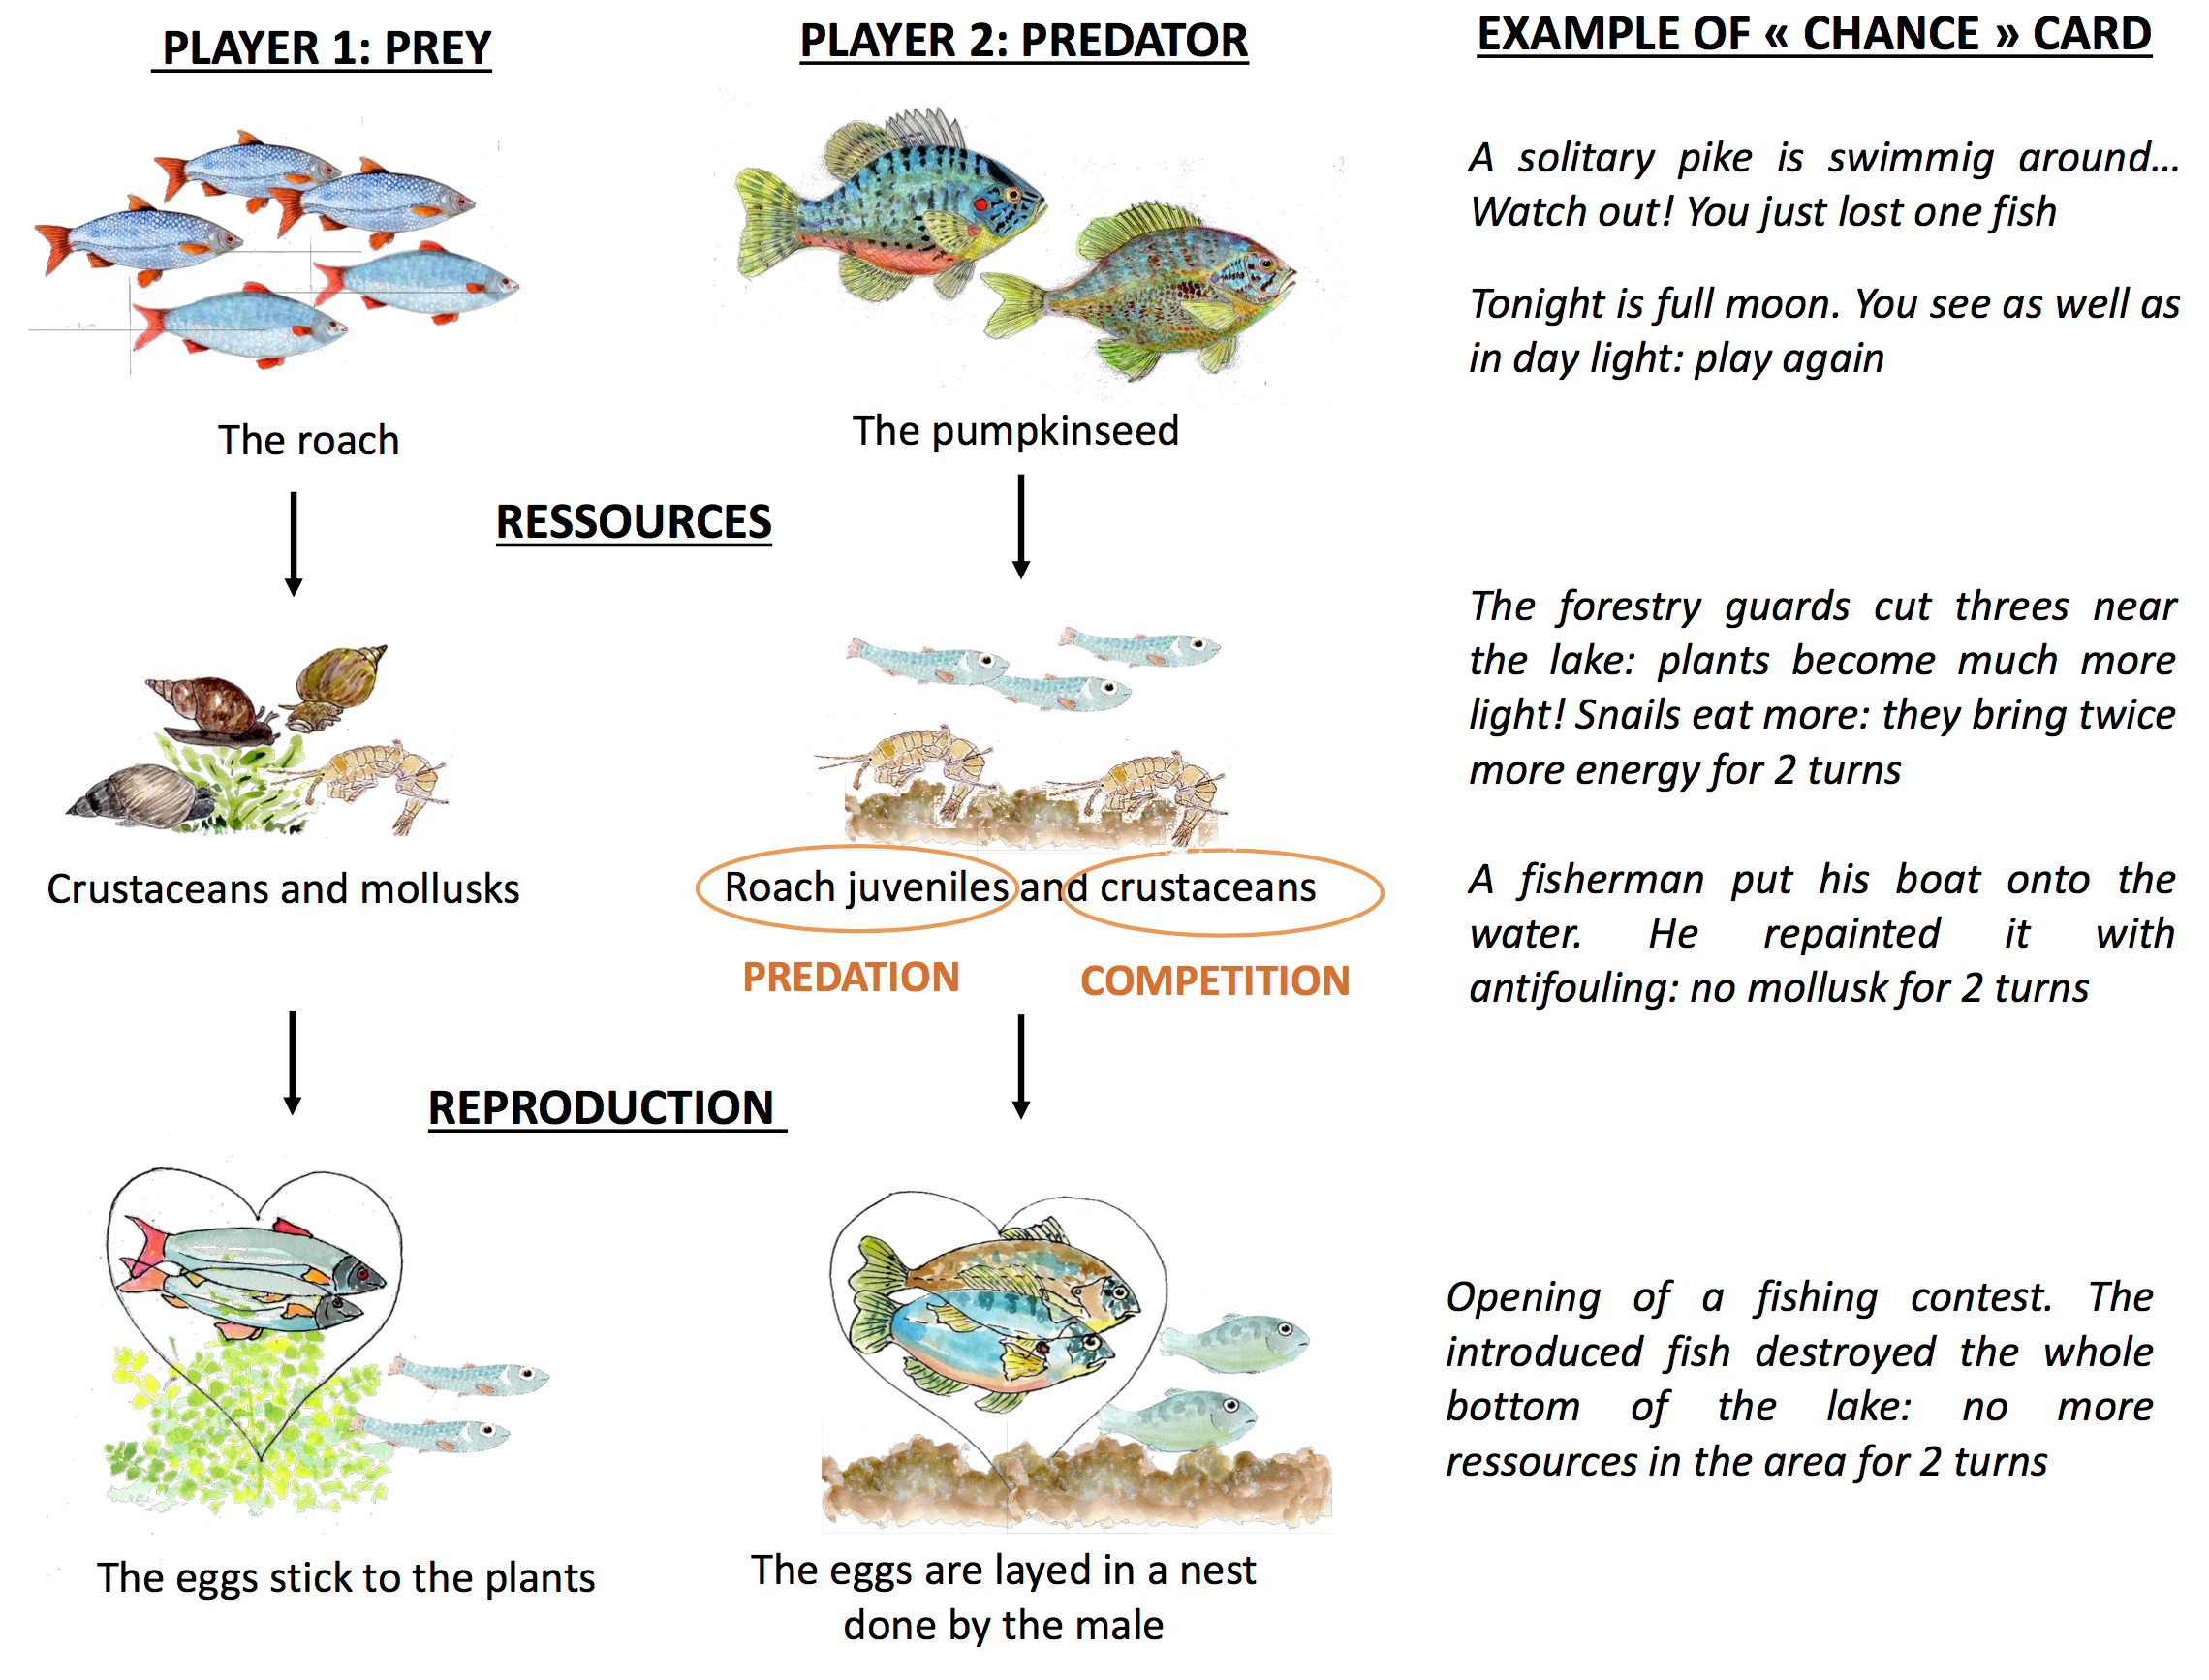
\includegraphics[width=\linewidth]{Figures/MediationEcotox/boardgame}
	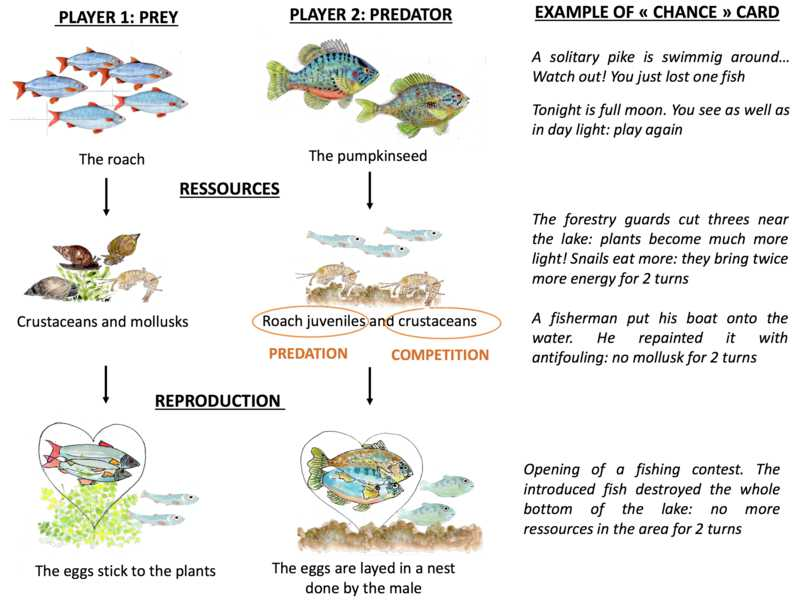
\includegraphics[width=\linewidth]{Figures/Final/C-mediationecotox-boardgame.jpg}
	\appcaption{\textbf{Principles of the board game.}\label{fig:app:mediationecotox:boardgame}}{\textbf{Principes du jeu de plateau.} Les espèces illustrées ici sont deux poissons européens commun de petite taille, le gardon (\textit{Rutilus rutilus}) comme proie et la perche soleil (\textit{Lepomis gibbosus}) comme prédateur. Nous donnons également des exemples de perturbations extérieures (cartes ``chance'').\label{fig:app:mediationecotox:boardgame}}
\end{figure}
%%%%%%%%%%%%%%

% Species: the roach (Rutilus rutilus) as a prey and the pumpkinseed (Lepomis gibbosus) as a predator, two common european small fish
% Illustration of a native european shoal fish (the roach) and of an invasive species (the pumpkinseed) with specific life history characteristics


\subsubsection{Computer-based game}{Jeu pour ordinateur}





\bpar{
The player controls an ecosytem with preys (the roach) and predators (the pumpkinseed). The objective of the game is to maintain the stability of the ecosystem. The concepts illustrated are population dynamic and ecosystem resilience.
}{
Dans le cas du jeu informatique, les joueurs\footnote{Le nombre de joueurs n'est pas spécifié, puisque le but est le maintien de la stabilité de l'ensemble de l'écosystème. Deux joueurs peuvent alors se répartirent les rôles de proie et prédateur, chacun jouant sur les paramètres qu'il contrôle pour stabiliser l'écosystème.} contrôlent un écosystème avec des proies (le gardon) et des prédateurs (la perche soleil). L'objectif est de maintenir la stabilité de l'écosystème et les concepts illustrés sont les dynamiques de population et la résilience d'un écosystème.
}


\bpar{
An agent-based model2 (ABM) for a simple prey-predator system isproposed as a basis of the computer game . ABM simulate the behavior and interactions between agents (fish) to reconstruct the population dynamic (bottom-up approach). Stochasticity is included with spatialized interactions (smoothed brownian motions), illustrating the randomisation of prey-predator interactions .Discrete dynamics consist in the following steps : (a) wandering of species in their prefered zone of the lake; (b) trophic interactions (fish-fish and fish-ressources) ; (c) renewing of fish (reproduction) and of ressources. The model parameters include reproduction rates, movement parameters, etc.
}{
Un modèle-basé agent pour un système proie-prédateur est proposé comme la base du jeu. L'ABM simule le comportement et les interactions entre agents (poissons) pour reconstruire la dynamique de population (approche \emph{bottom-up}). La stochasticité est prise en compte via les interactions spatialisées (rencontre aléatoires entre des mouvements browniens lissés), illustrant le caractère aléatoire des interactions proie-prédateur. La dynamique discrète est composée par les points suivants : (a) mouvement des individus ; (b) interactions trophiques ; (c) renouvellement de la population (reproduction). Les paramètres du modèle incluent taux de reproduction et de prédation, et de survie pour le prédateur, ainsi que les paramètres de mouvement.
}


\bpar{
(Netlogo software). Large-scale model exploration and calibration are currently running (Using OpenMole model exploration platform~\cite{reuillon2013openmole} to explore the NetLogo implementation which source code is openly available on the repository of the project at https://github.com/JusteRaimbault/MediationEcotox) in order to find parameter ranges at which ecosystem is in equilibrium1. Systematic exploration of parameter space using OpenMole software3, to verify theoretical average trajectories in phase space, which allows analytical and numerical determination of initial position (attractor) and justify the use of this system for the game.
}{
Le modèle est implémenté en NetLogo, ce qui permet son utilisation en ligne par l'intermédiaire de NetLogoweb\footnote{L'implémentation ouverte est disponible sur le dépôt du projet à \url{https://github.com/JusteRaimbault/MediationEcotox}.}. Le modèle est exploré par l'intermédiaire d'OpenMole~\cite{reuillon2013openmole}, afin de vérifier la position théorique des attracteurs et des trajectoires moyennes dans l'espace des phases. Nous obtenons sur une grille de l'espace des paramètres (taux de reproduction de la proie, taux de prédation, taux de survie du prédateur) une bonne correspondance entre les attracteurs théoriques et les attracteurs simulés. La Fig.~\ref{fig:app:mediationecotox:phasediags} illustre des diagrammes de phase obtenus par les simulations. La connaissance des attracteurs permet d'utiliser le modèle pour le jeu.
}


%%%%%%%%%%%%
\begin{figure}
	%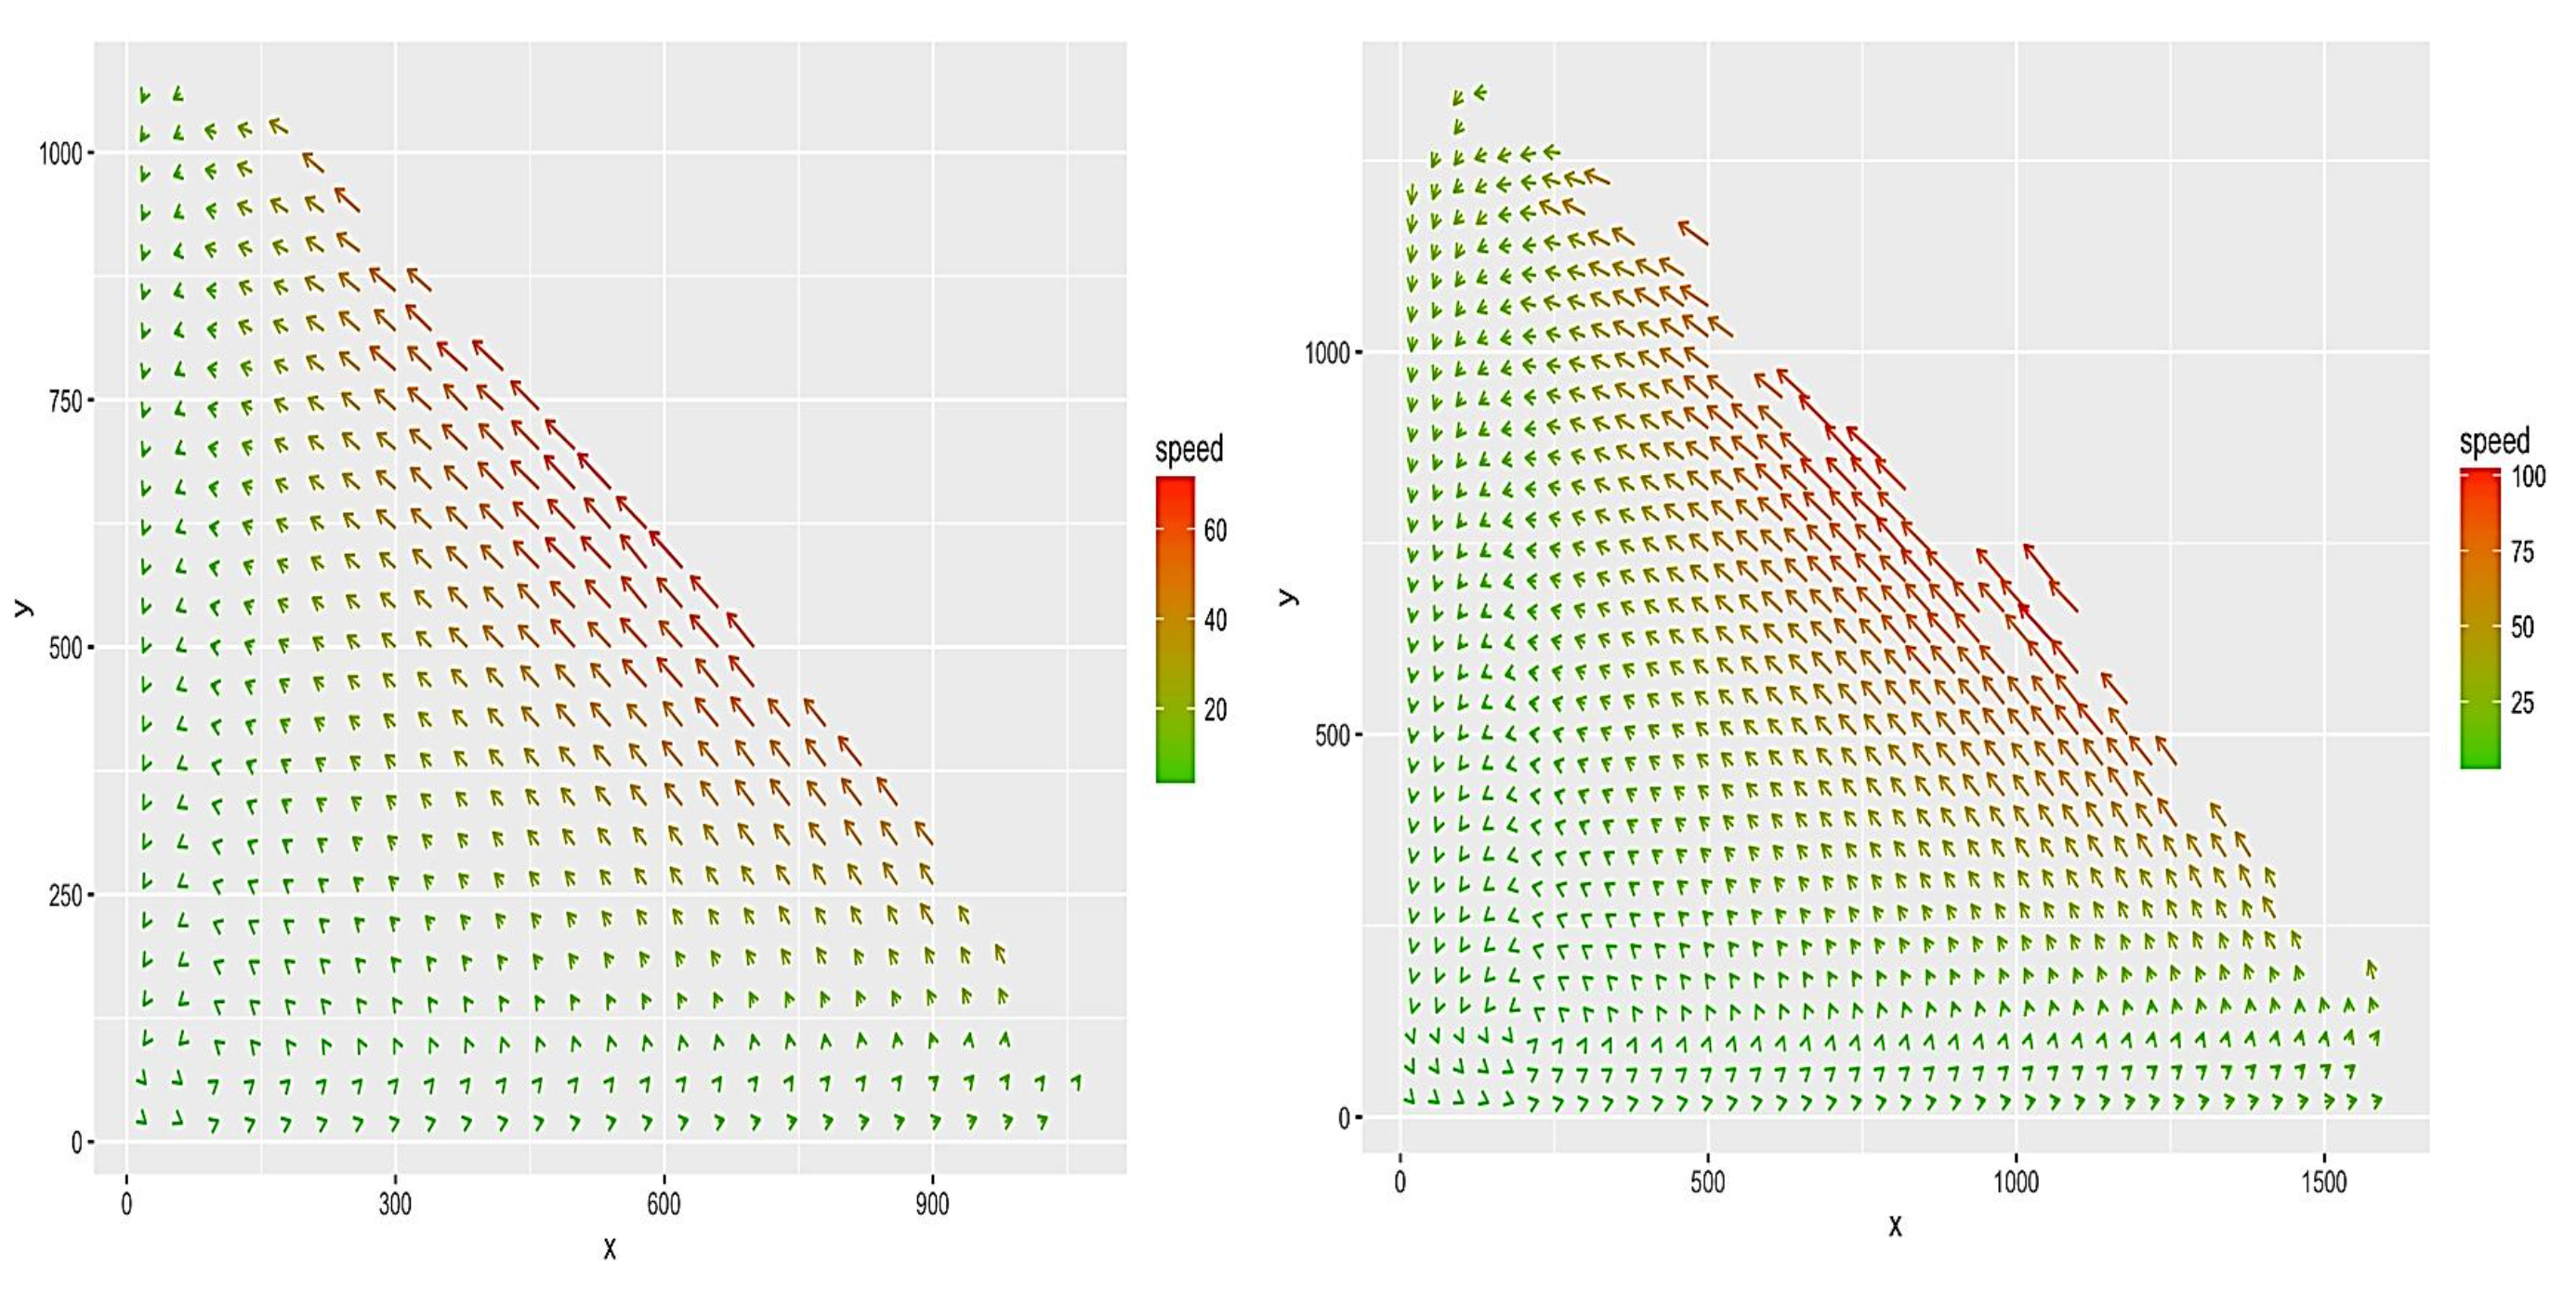
\includegraphics[width=\linewidth]{Figures/MediationEcotox/phasediags.png}
	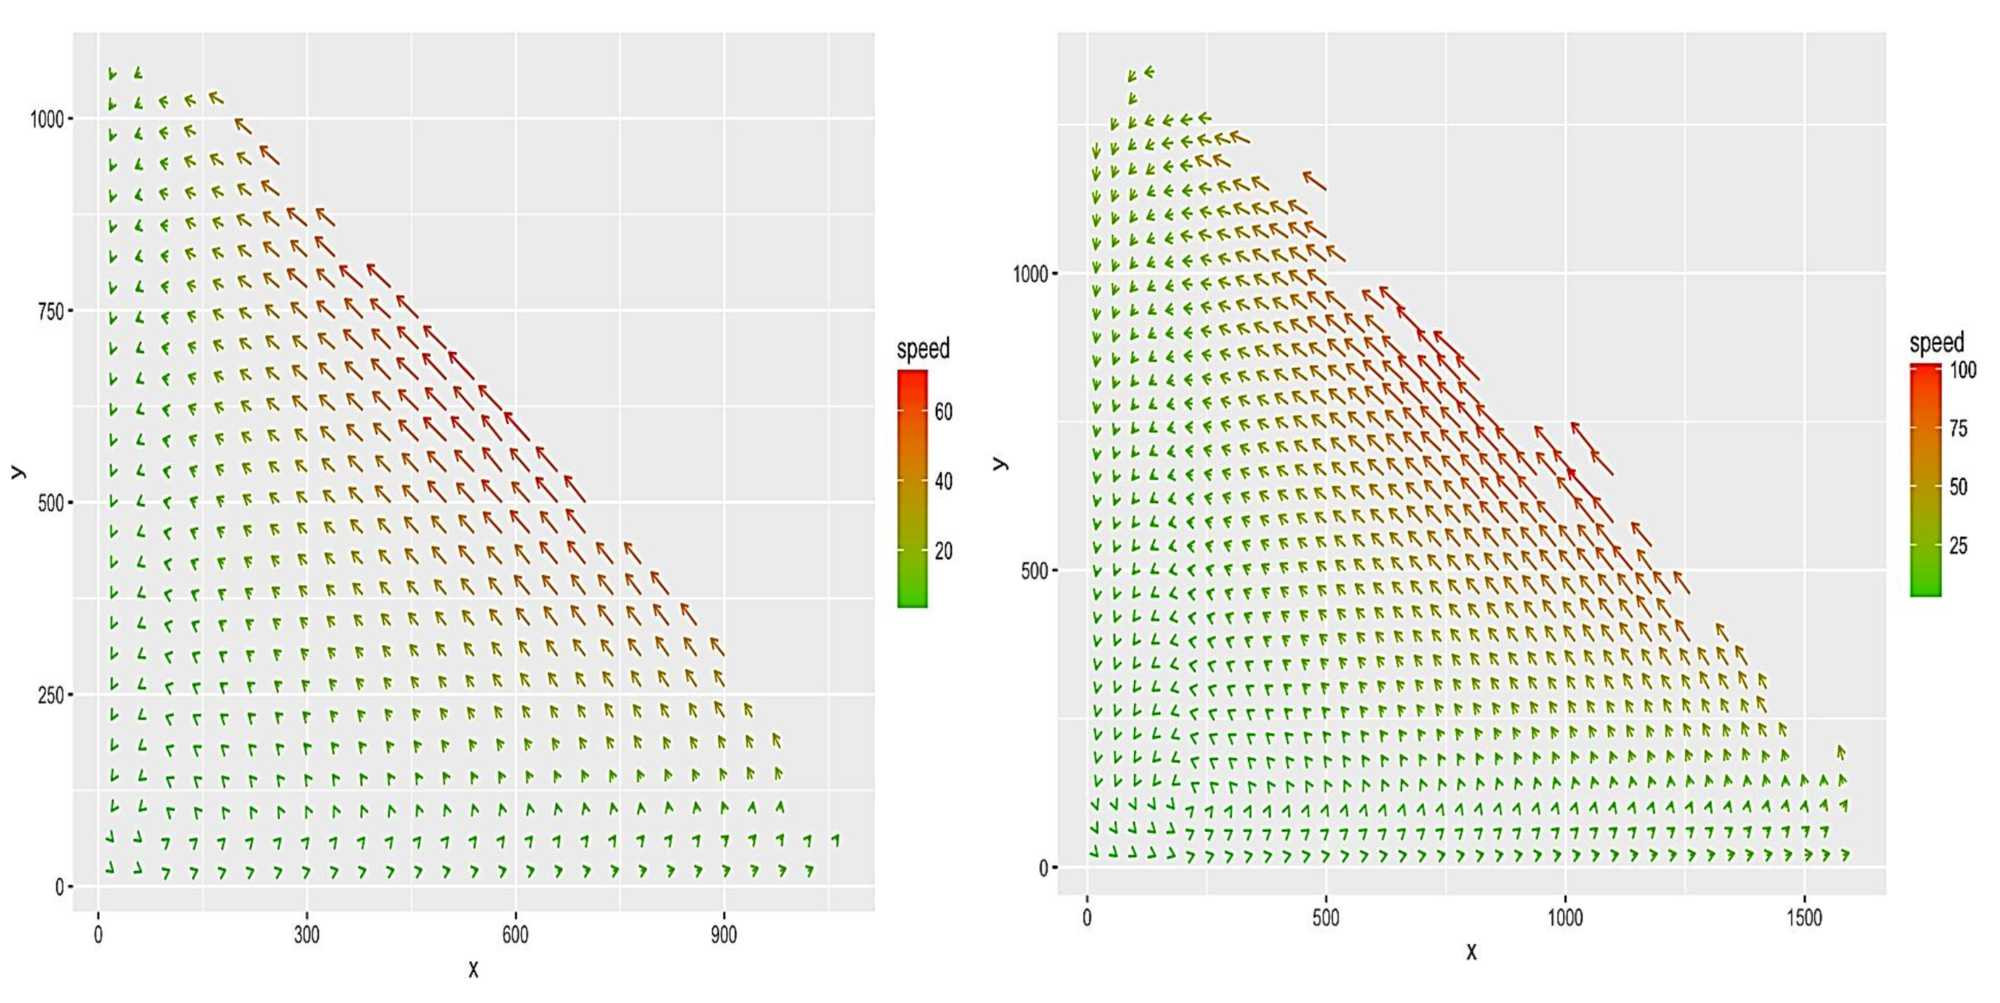
\includegraphics[width=\linewidth]{Figures/Final/C-mediationecotox-phasediags.jpg}
	\appcaption{\textbf{Examples of phase diagrams of the prey-predator model.}\label{fig:app:mediationecotox:phasediags}}{\textbf{Exemples de diagrammes de phase du modèle proie-prédateur.} L'exploration systématique permet de vérifier l'expression théorique des trajectoires moyennes dans l'espace des phases. Les graphes donnent les portraits de phase des deux populations (x/y), pour deux points de l'espace des paramètres.\label{fig:app:mediationecotox:phasediags}}
\end{figure}
%%%%%%%%%%%%

%  The figures show estimated average trajectories for two points in parameter space.


\bpar{
The player starts the game with a stable ecosystem: the initial position is the attractor. The button « one turn » makes the ecosystem evolve during 50 time steps. The player sees the changes in the fish populations simustaneoulsy on the screen. The trajectory can be corrected towards the attractor in the phase space by changing the parameters of the model (predator survival, prey reproduction and hunting behavior). External events randomly perturbate the ecosystem. The game includes 5 levels of difficulty based on event strength
%The equilibrium will constitute the default state of the system without user control. User interactions are then integrated after each turn, at given time intervals (one month, when one time step is 6h for example). It allows the system to evolve in-between. During this time frame, the players observe the consequences of its actions and the reaction of the ecosystem to external events. Further developments will consist in model refinment and user latitude adjustements thanks to player feedbacks.
}{
En effet, le jeu commence à un écosystème à l'équilibre, c'est-à-dire que les valeurs des populations sont fixées à l'attracteur non nul. Un bouton pour jouer un tour fait évoluer l'écosystème sur 50 pas de temps. Le joueur observe alors la trajectoire des populations. La trajectoire peut alors être corrigée par le joueur par action sur les paramètres du modèle (survie du prédateur, reproduction de la proie, prédation) et donc la position de l'attracteur. Des évènement extérieur aléatoires perturbent les populations, et conjointement au bruit contribuent à déstabiliser l'écosystème, qui peut passer sur des orbites plus proches de l'effondrement (disparition d'une espèce). Le jeu inclut 5 niveaux de difficultés, basés sur la force des perturbations.
}

% note : serait cool d'agir sur l'amplitude du bruit également ?
% IDEE : calculer proba de collapse selon position, attracteur et bruit (doit pas pouvoir faire analytique, besoin openmole) -> fixer difficulté selon proba avec seuils.

%%%%%%%%%%%%
\begin{figure}
	%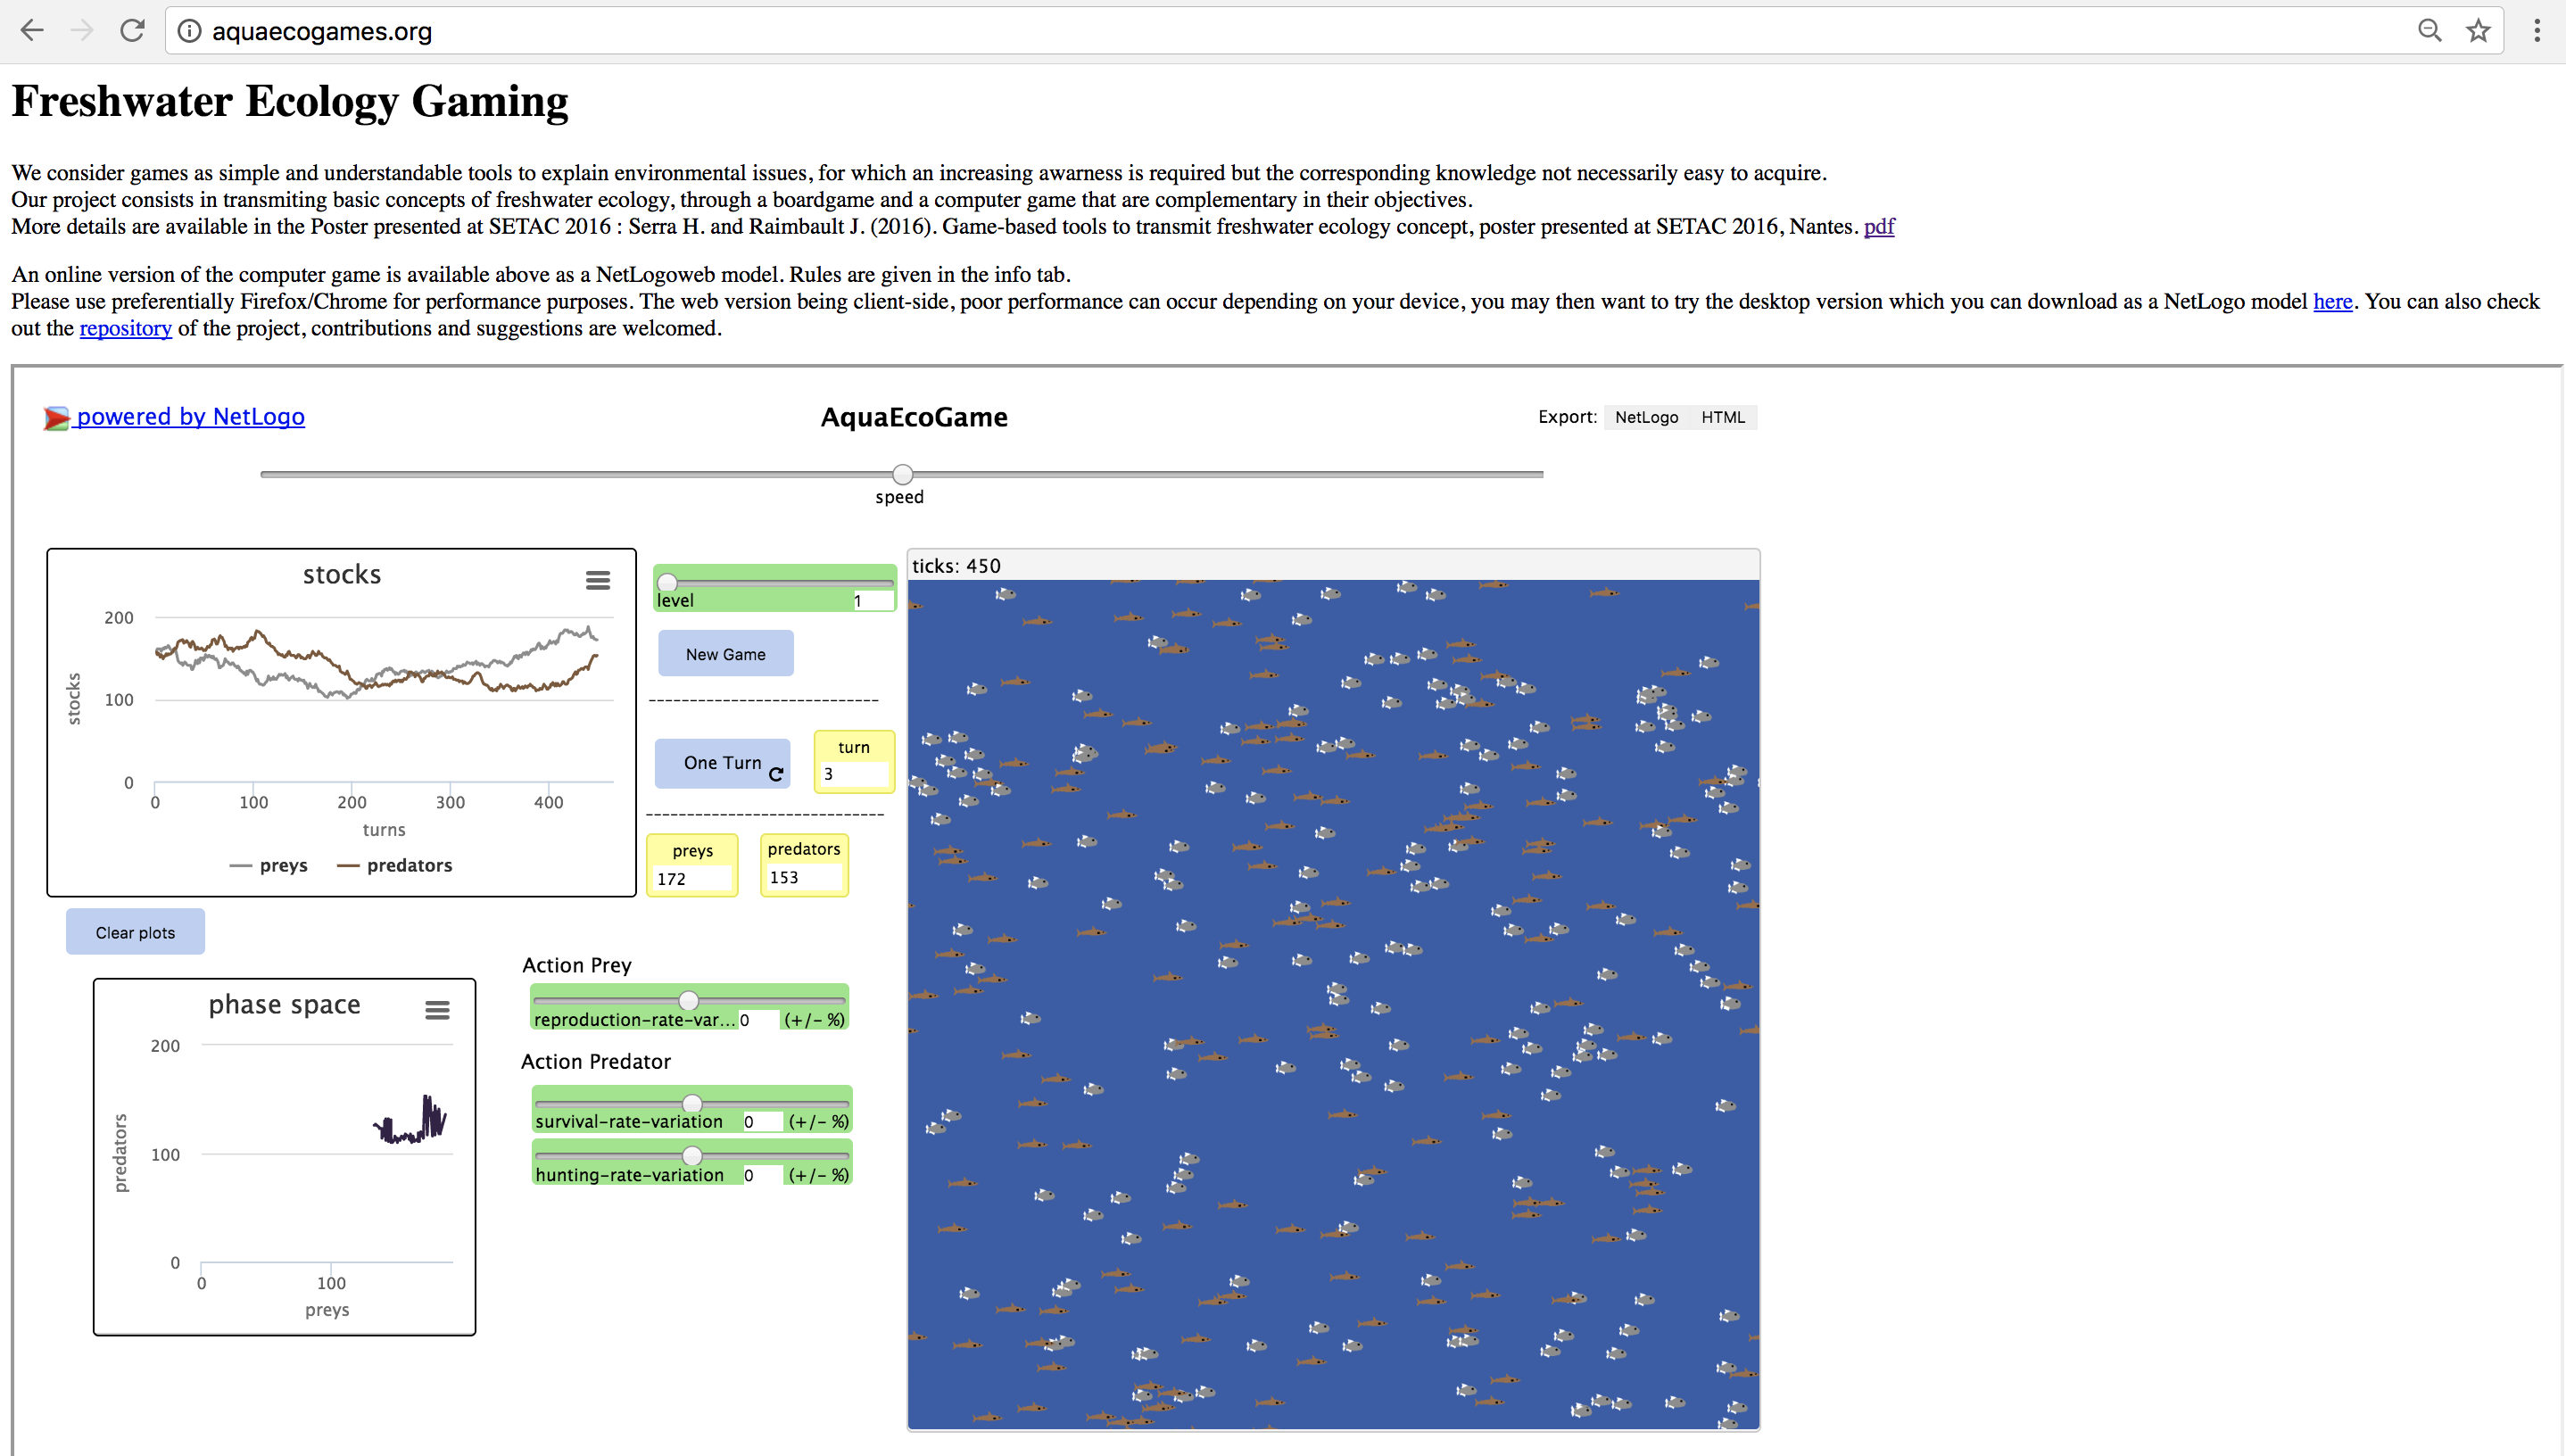
\includegraphics[width=\linewidth]{Figures/MediationEcotox/webpage.png}
	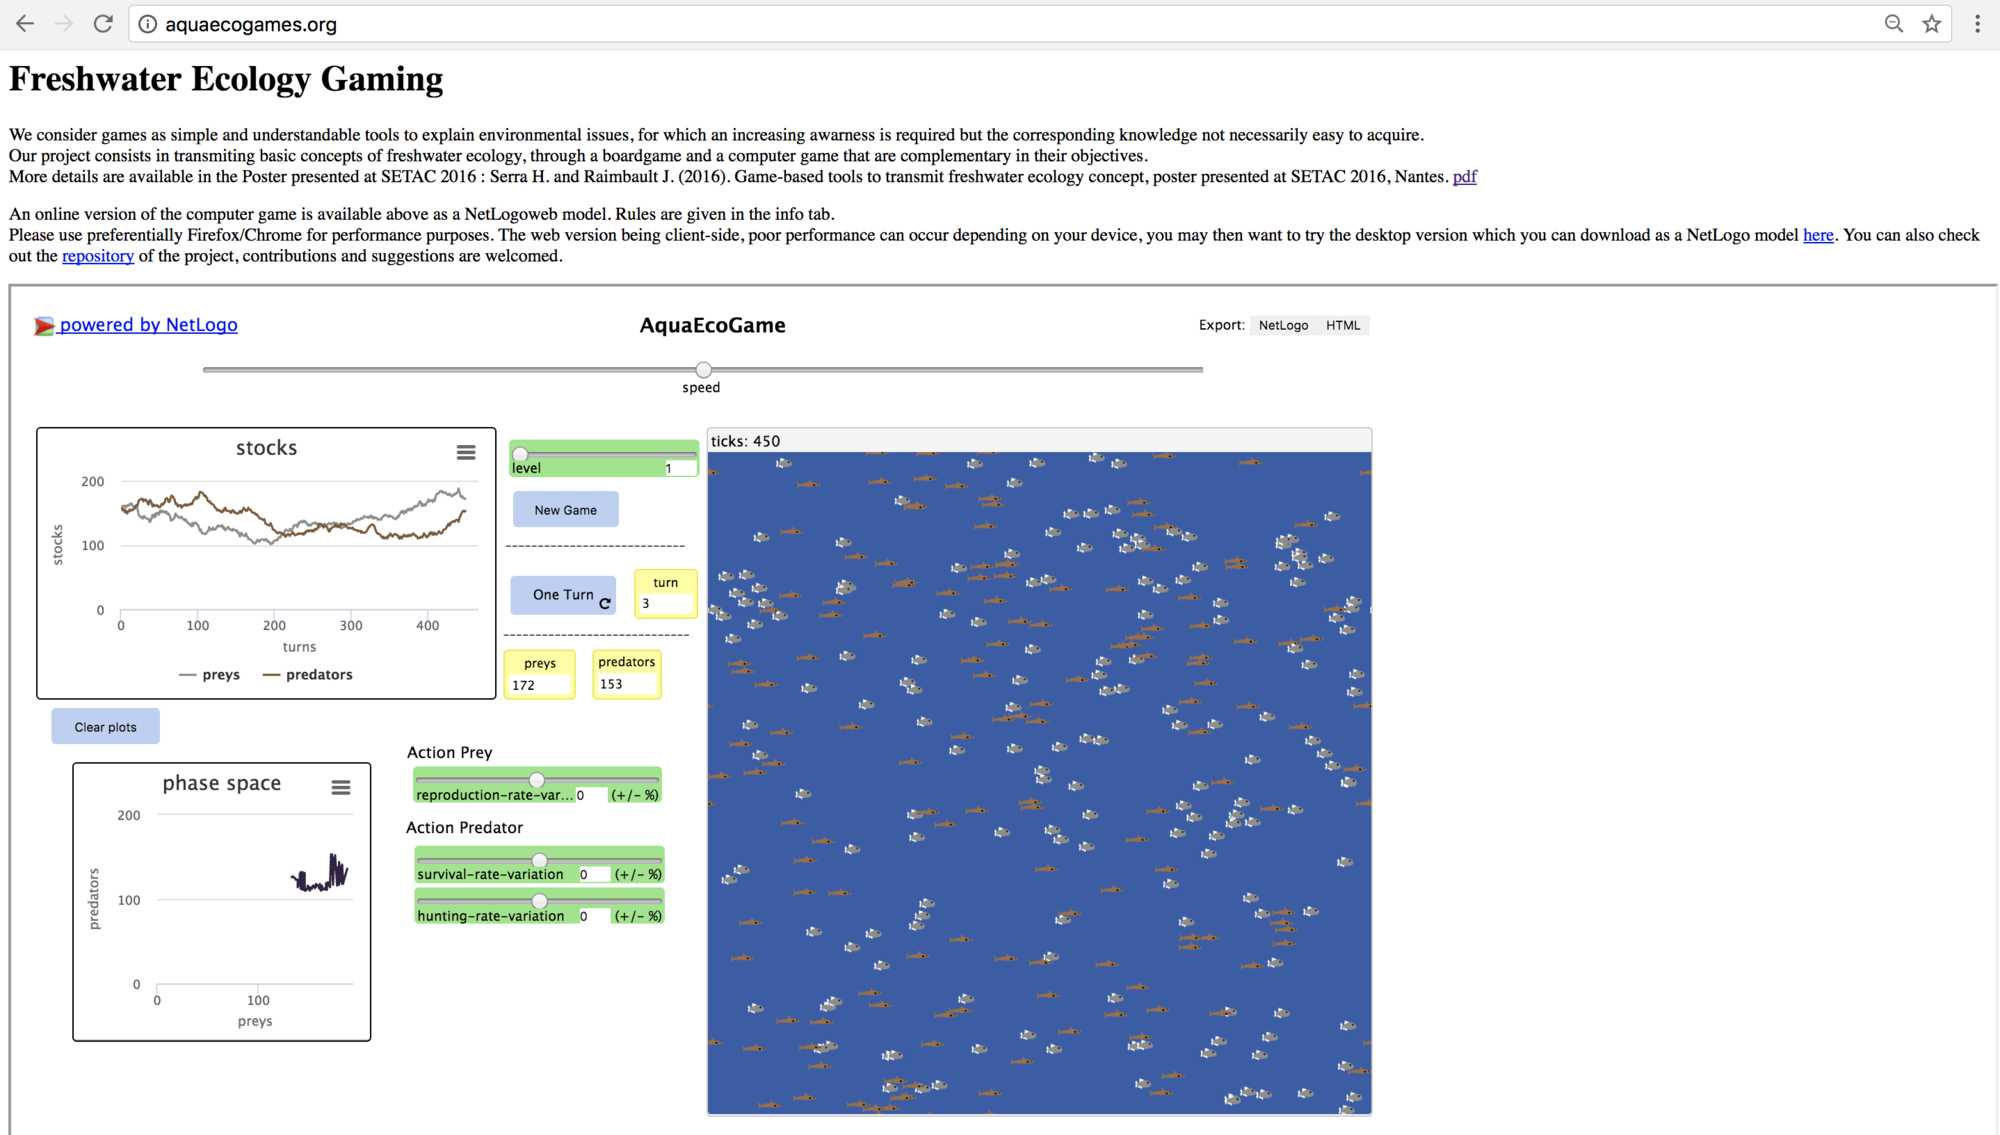
\includegraphics[width=\linewidth]{Figures/Final/C-mediationecotox-webpage.jpg}
	\appcaption{\label{fig:app:mediationecotox:webpage}}{\textbf{Capture de l'application web qui implémente le jeu informatique.} Le contexte, la documentation et les liens vers les ressources sont brièvement rappelés, et NetLogoweb est inclus dans la page pour l'interface du jeu.\label{fig:app:mediationecotox:webpage}}
\end{figure}
%%%%%%%%%%%%


\bpar{
available at http://aquaecogames.org/
}{
La version NetLogoweb du jeu (qui ne contient que les graphiques minimaux à cause des restrictions par rapport à NetLogo natif) est disponible en ligne à \url{http://aquaecogames.org/}. Une capture d'écran de l'application web est montrée en Fig.~\ref{fig:app:mediationecotox:webpage}.
}




\subsection{Discussion}{Discussion}


%Demonstration of the proof-of-concept: the prototypes are available for testing
% Both game are complementary as they integrate different time scales and illustrate diverse basic concepts of aquatic ecology
% No knowledge in aquatic ecology is needed to play both games: wide possibilities in targeted audiences
% The methodology is flexible and adaptable: 
% - On-going development of the games
% - Refinements and changes are easy to integrate in new versions of the games

%Short term perspectives:
% Next step of the project: test the games and gather player feedbacks 
%  - do players like the games?
%  - Identification of potential players (children, school/university, family, adults...) and adaptation of the games accordingly (simplication/complexification) Long term perspectives:
% Potential uses of the games as educational tools (with educative support) or sensibilisation tools (e.g. adapting the species and perturbations)
% Funding and diffusion of the board game through crowdfunding plateforms and game festivals
% Diffusion of the computer-based game: open online access through Netlogoweb and development of mobile applications

\bpar{
A prototype of each game is currently available for testing and refinements are expected while experiencing the games. In a short term, next versions of the games will be developed after player feedback and will include the aesthetic design of the games and refined processes parameters. Mid-term and long-term objectives are oriented towards an online version of the computer game as described before, and the use of crowdfunding platforms to offer and diffuse the board game.
}{
Un prototype pour chaque jeu est disponible actuellement pour des tests et des ajustements sont prévus en fonction des retours d'expérience. A court terme, les prochaines versions des jeux seront développées selon le retour des joueurs et incluront une conception esthétique ainsi que des processus plus fins. Les objectifs à moyen et long terme s'orientent vers un développement natif de l'application web et l'utilisation de plateformes de financement participatif pour diffuser le jeu de plateau.
}


\bpar{
The very first objective of our games remains to be entertaining, keeping in mind that the ludic rather than pedagogical aspects are central in the success of such game-based media. If players forget that the game is about ecology, our precise objective is reached. It would mean that the underlying scientific concepts are clearly understood.
}{
Il faut garder à l'esprit que le caractère ludique plutôt que pédagogique est central dans le succès de tels media basés sur les jeux. Si les joueurs oublient que le jeu est à propos d'un problème écologique, l'objectif est précisément atteint, puisque cela signifierait que les concepts scientifiques sous-jacents sont clairement compris.
}



\stars








